\documentclass[11pt,a4paper]{article}
\usepackage[margin=2.2cm]{geometry}
\usepackage{amsmath,amssymb,graphicx,booktabs,siunitx,caption,authblk,hyperref,microtype}
\captionsetup{font=small,labelfont=bf}
\sisetup{detect-all}
% auto-generated by scripts/build_paper.py from results/summary.json - do not edit
\newcommand{\PZt}{53.9}
\newcommand{\PZtOhm}{494}
\newcommand{\PBW}{9.69}
\newcommand{\PPow}{0.97}
\newcommand{\PPk}{0.09}
\newcommand{\PInOne}{15.8}
\newcommand{\PInFive}{15.4}
\newcommand{\PInTen}{19.0}
\newcommand{\PIrms}{1.59}
\newcommand{\PIrmsTot}{1.75}
\newcommand{\PFlat}{8.0}
\newcommand{\PInAvg}{16.2}
\newcommand{\PFom}{4935}
\newcommand{\Vin}{0.27}
\newcommand{\Vout}{0.66}
\newcommand{\Vn}{0.44}
\newcommand{\IOne}{112}
\newcommand{\ITwo}{211}
\newcommand{\IThree}{663}
\newcommand{\IF}{99}
\newcommand{\GmOne}{1.75}
\newcommand{\GmTwo}{2.48}
\newcommand{\GmThree}{6.41}
\newcommand{\GmF}{1.54}
\newcommand{\RtNom}{751}
\newcommand{\Ro}{1048}
\newcommand{\ITot}{970}
\newcommand{\BZt}{38.0}
\newcommand{\BZtOhm}{79}
\newcommand{\BPk}{11.8}
\newcommand{\BFpk}{18.9}
\newcommand{\BFlat}{7.1}
\newcommand{\BPow}{1.32}
\newcommand{\BInOne}{33.3}
\newcommand{\BInFive}{30.8}
\newcommand{\BInTen}{26.5}
\newcommand{\BInFifteen}{24.2}
\newcommand{\BIrmsTot}{10.3}
\newcommand{\BITwo}{661}
\newcommand{\BIOne}{4.8}
\newcommand{\BGmTwo}{5.14}
\newcommand{\BGdsOne}{2.88}
\newcommand{\BVin}{0.50}
\newcommand{\BFom}{426}
\newcommand{\BMZt}{35.2}
\newcommand{\BMPow}{2.29}
\newcommand{\BMPk}{7.0}
\newcommand{\BMInFive}{53.8}
\newcommand{\GainImp}{15.9}
\newcommand{\NoiseRatio}{2.0}
\newcommand{\PowSave}{27}
\newcommand{\TuneMin}{5.56}
\newcommand{\TuneMax}{9.73}
\newcommand{\TuneRatio}{1.75}
\newcommand{\VtOneDb}{0.30}
\newcommand{\RtMin}{160}
\newcommand{\RtMaxOne}{951}
\newcommand{\IrmsMin}{1.16}
\newcommand{\PkMax}{4.4}
\newcommand{\VtMax}{0.44}
\newcommand{\VtNom}{0.28}
\newcommand{\AIRs}{497}
\newcommand{\AIgm}{1.54}
\newcommand{\AILA}{0.3}
\newcommand{\AIQA}{0.00}
\newcommand{\AIRtA}{751}
\newcommand{\AILB}{5.5}
\newcommand{\AIQB}{0.07}
\newcommand{\AIRtB}{1238}
\newcommand{\AILC}{14.2}
\newcommand{\AIQC}{0.16}
\newcommand{\AIRtC}{2284}
\newcommand{\AILD}{22.0}
\newcommand{\AIQD}{0.23}
\newcommand{\AIRtD}{4695}
\newcommand{\LoopTzero}{10.4}
\newcommand{\LoopPMg}{103}
\newcommand{\LoopPMl}{68}
\newcommand{\LoopPMlCpd}{52}
\newcommand{\LoopFuMin}{1.7}
\newcommand{\LoopFuMax}{3.5}
\newcommand{\PvtBwMin}{8.03}
\newcommand{\PvtBwMax}{11.40}
\newcommand{\PvtPkMin}{0.06}
\newcommand{\PvtPkMax}{2.36}
\newcommand{\PvtBwTMin}{7.94}
\newcommand{\PvtBwTMax}{10.67}
\newcommand{\PvtPkTMin}{0.06}
\newcommand{\PvtPkTMax}{0.40}
\newcommand{\PvtZtMin}{52.84}
\newcommand{\PvtZtMax}{54.64}
\newcommand{\PvtPMin}{0.72}
\newcommand{\PvtPMax}{1.13}
\newcommand{\ZtExact}{500}
\newcommand{\ZtApprox}{524}
\newcommand{\Tzero}{4.18}
\newcommand{\AOne}{5.6}
\newcommand{\Mratio}{2.59}
\newcommand{\Fz}{6.1}
\newcommand{\Fp}{7.1}
\newcommand{\CapCin}{121}
\newcommand{\CapCn}{7}
\newcommand{\CapCo}{76}
\newcommand{\CapCg}{35}
\newcommand{\CapCm}{6}
\newcommand{\CapCgg}{0}
\newcommand{\ModelRmsNom}{0.37}
\newcommand{\ModelRmsMax}{1.00}
\newcommand{\ModelRmsLow}{0.50}
\newcommand{\ModelMaxLow}{0.9}
\newcommand{\ModelMaxAll}{3.2}
\newcommand{\EyePTenH}{53.6}
\newcommand{\EyePTenPct}{87}
\newcommand{\EyePTenW}{93}
\newcommand{\EyePTenAmp}{61.5}
\newcommand{\EyeBTenH}{7.8}
\newcommand{\EyeBTenPct}{87}
\newcommand{\EyeBTenW}{97}
\newcommand{\EyeBTenAmp}{9.0}
\newcommand{\EyePTwH}{53.5}
\newcommand{\EyePTwPct}{88}
\newcommand{\EyePTwW}{92}
\newcommand{\EyePTwAmp}{61.1}
\newcommand{\EyeBTwH}{7.7}
\newcommand{\EyeBTwPct}{99}
\newcommand{\EyeBTwW}{53}
\newcommand{\EyeBTwAmp}{7.8}
\newcommand{\ZoutB}{79}
\newcommand{\ZoutBF}{79}
\newcommand{\ZoutP}{238}
\newcommand{\ZoutBMax}{622}
\newcommand{\SensIpp}{24.6}
\newcommand{\SensdBm}{-18.1}
\newcommand{\SpiralSide}{136}
\newcommand{\SpiralArea}{0.018}
\newcommand{\AIArea}{138}
\newcommand{\AreaRatio}{134}
\newcommand{\OvA}{1.2}
\newcommand{\OvB}{2.6}
\newcommand{\OvC}{6.7}
\newcommand{\OvBwB}{7.0}
\newcommand{\OvBwC}{2.3}
\newcommand{\LdResLight}{11.53}
\newcommand{\LdAiLight}{9.72}
\newcommand{\LdRatioLight}{0.84}
\newcommand{\LdResHeavy}{2.33}
\newcommand{\LdAiHeavy}{3.08}
\newcommand{\LdRatioHeavy}{1.32}
\newcommand{\LdRatioMid}{1.10}
\newcommand{\NsMOne}{31}
\newcommand{\NsMTwo}{24}
\newcommand{\NsMThree}{13}
\newcommand{\NsMf}{13}
\newcommand{\NsMt}{8}
\newcommand{\NsMThreeB}{4}
\newcommand{\NsRn}{7}
\newcommand{\NsBMOne}{64}
\newcommand{\McN}{200}
\newcommand{\McBwMean}{9.55}
\newcommand{\McBwStd}{0.55}
\newcommand{\McBwMin}{6.88}
\newcommand{\McBwMax}{10.94}
\newcommand{\McBwTMean}{9.44}
\newcommand{\McBwTStd}{0.41}
\newcommand{\McBwTMin}{7.16}
\newcommand{\McBwTMax}{9.96}
\newcommand{\McPkMax}{2.64}
\newcommand{\McPkTMax}{0.50}
\newcommand{\McZtMean}{54.0}
\newcommand{\McZtStd}{0.89}
\newcommand{\McPStd}{0.026}
\newcommand{\McYieldFixed}{78}
\newcommand{\McYieldTrim}{86}
\newcommand{\McPkYieldFixed}{91}
\newcommand{\McPkYieldTrim}{100}
\newcommand{\McVtMin}{0.00}
\newcommand{\McVtMax}{0.36}
\newcommand{\DgRmsDrawn}{13.5}
\newcommand{\DgRmsFitDrawn}{4.1}
\newcommand{\DgRmsMOne}{5.0}
\newcommand{\DgRmsMTwoB}{6.5}
\newcommand{\DgRmsLoss}{4.3}
\newcommand{\DgRmsBestL}{3.5}
\newcommand{\DgRsBestL}{108}
\newcommand{\DgRmsNoL}{1.6}
\newcommand{\DgVgNoL}{0.50}
\newcommand{\DgIdNoL}{137}
\newcommand{\DgPwrNoL}{0.27}
\newcommand{\DgLfMax}{30}
\newcommand{\DgRmsTwoFour}{4.1}
\newcommand{\DgSatMax}{0.00}
\newcommand{\DgVdsRatioMax}{1.99}
\newcommand{\DgNScreen}{30}
\newcommand{\DgPkMin}{6.9}
\newcommand{\DgEqNine}{15}
\newcommand{\RgZt}{54.0}
\newcommand{\RgBw}{3.6}
\newcommand{\RgPk}{0.5}
\newcommand{\RgPow}{0.09}
\newcommand{\RgInFive}{8.4}
\newcommand{\RgIrms}{0.52}
\newcommand{\RgFom}{19959}
\newcommand{\RgGbw}{1.8}
\newcommand{\RbZt}{44.6}
\newcommand{\RbBw}{30.8}
\newcommand{\RbPk}{0.0}
\newcommand{\RbPow}{0.26}
\newcommand{\RbInFive}{17.1}
\newcommand{\RbIrms}{2.95}
\newcommand{\RbFom}{20250}
\newcommand{\RbGbw}{5.3}
\newcommand{\RgLf}{5.0}
\newcommand{\RbLf}{1.25}
\newcommand{\RgRs}{43}
\newcommand{\RbRs}{43}
\newcommand{\PFomP}{4935}
\newcommand{\PGbw}{4.8}
\newcommand{\BwRatioGain}{2.7}
\newcommand{\DcLimit}{500}
\newcommand{\PrLimit}{10}
\newcommand{\DcPow}{1.05}
\newcommand{\DcPowAdd}{82}
\newcommand{\DcImfDark}{108}
\newcommand{\DcIdccDark}{12}
\newcommand{\DcBwDark}{9.86}
\newcommand{\DcZtDark}{53.4}
\newcommand{\DcFloDark}{111}
\newcommand{\DcBwFive}{9.25}
\newcommand{\DcZtFive}{0.6}
\newcommand{\DcImfFive}{96}
\newcommand{\DcBwThree}{9.64}
\newcommand{\DcImfThree}{104}
\newcommand{\DcBwHund}{9.78}
\newcommand{\DcFloMax}{1.4}
\newcommand{\DcPkHfMax}{0.0}
\newcommand{\DcPkLfMax}{1.2}
\newcommand{\PrBwHundred}{2.3}
\newcommand{\PrBwFifty}{7.0}
\newcommand{\DcInFive}{16.3}
\newcommand{\DcInFiveThree}{17.7}
\newcommand{\DcNoisePct}{6}
\newcommand{\ShotThree}{9.8}
\newcommand{\DcPmMin}{81}
\newcommand{\DcFuMin}{108}
\newcommand{\DcFuMax}{1.5}
\newcommand{\DcTzMax}{38}
\newcommand{\DcTzMin}{18}
\newcommand{\DcSettle}{0.6}
\newcommand{\DcDip}{238}
\newcommand{\DcErr}{2}
\newcommand{\PrDrop}{264}
\newcommand{\PrEyeZero}{87}
\newcommand{\PrEyeWZero}{93}
\newcommand{\PrEyeHund}{28}
\newcommand{\PrEyeWHund}{42}
\newcommand{\PrEyeThree}{70}
\newcommand{\PrEyeWThree}{83}
\newcommand{\DcEyeZero}{87}
\newcommand{\DcEyeWZero}{93}
\newcommand{\DcEyeHund}{87}
\newcommand{\DcEyeWHund}{93}
\newcommand{\DcEyeThree}{87}
\newcommand{\DcEyeWThree}{93}
\newcommand{\DcPvtIdccMax}{27}
\newcommand{\DcPvtBwMin}{7.1}
\newcommand{\DcPvtBwMinB}{8.3}
\newcommand{\DcPvtN}{13}
\newcommand{\DcMcN}{100}
\newcommand{\DcMcBwMean}{9.42}
\newcommand{\DcMcBwStd}{0.88}
\newcommand{\DcMcBwMin}{6.14}
\newcommand{\DcMcBwDarkMin}{8.95}
\newcommand{\DcMcPrDarkMin}{6.75}
\newcommand{\DcMcIdccMed}{12}
\newcommand{\DcMcIdccMax}{161}
\newcommand{\DcMcImfStd}{25}
\newcommand{\DcMcPkMax}{3.5}
\newcommand{\DcMcPrPkMax}{2.2}
\newcommand{\DcMcZtStd}{1.1}
\newcommand{\DcMcPrZtStd}{1.2}
\newcommand{\DcMcImfDarkStd}{19}
\newcommand{\DcMcPkN}{21}
\newcommand{\DcTrBwMin}{9.6}
\newcommand{\DcTrBwThree}{8.5}
\newcommand{\DcTrPkThree}{0.7}

\makeatletter\let\tableinput\@@input\makeatother % expandable \input for table bodies

\title{An Inductorless, Bandwidth-Tunable Current-Mirror Transimpedance Amplifier with Active-Inductor Feedback in 90\,nm CMOS}
\author{Shreyas S}
\affil{Department of Electronics and Communication Engineering, R V College of Engineering, Bengaluru, India}
\date{}

\begin{document}
\maketitle

\begin{abstract}
A current-mirror transimpedance amplifier (TIA) that uses a \SI{2.4}{nH} spiral inductor as global feedback is re-examined with a BSIM4 device model, and an inductorless replacement is proposed. Re-simulated as drawn with the 90\,nm Predictive Technology Model, the published circuit delivers \BZt\,dB$\Omega$ with an \BPk\,dB resonance peak at \BFpk\,GHz, because its bias leaves the common-gate device in triode. The proposed circuit keeps the common-gate input and the mirror, biases them as a flipped-voltage-follower stage, and closes the loop with a source follower whose gate is driven from the output through a MOS resistor controlled by one voltage, $V_{tune}$. The follower and its gate network form a lossy active inductor. In simulation at \SI{1}{V} the TIA reaches \PZt\,dB$\Omega$ and \PBW\,GHz with \PPk\,dB peaking, \PInFive\,pA/$\sqrt{\text{Hz}}$ input-referred noise at \SI{5}{GHz} and \PPow\,mW, for a \SI{50}{fF} photodiode and a \SI{30}{fF} load. $V_{tune}$ moves the $-3$\,dB bandwidth from \TuneMin\ to \TuneMax\,GHz with less than \SI{1}{dB} peaking and removes the peaking that process, voltage and temperature shifts introduce (from \PvtPkMax\,dB to at most \PvtPkTMax\,dB over fifteen conditions). Relative to the re-simulated baseline the gain is \GainImp\,dB higher, the noise density at \SI{5}{GHz} is \NoiseRatio\ times lower and the power is \PowSave\,\% lower, and the feedback element is estimated to be two orders of magnitude smaller than the spiral. The study also reports what the active inductor does not do: it does not raise the maximum bandwidth above that of plain follower feedback at light loads, and the input stage overloads at an average photocurrent of a few tens of microamperes.
\end{abstract}

\noindent\textbf{Keywords:} transimpedance amplifier; active inductor; current mirror; flipped voltage follower; optical receiver; bandwidth tuning; 90\,nm CMOS.

\section{Introduction}
The transimpedance amplifier sets the sensitivity and much of the bandwidth of an optical receiver front end \cite{razavi,sackinger}. Current-mirror TIAs are attractive at supplies of \SI{1}{V} and below because the signal stays in the current domain until the output node, and several low-power designs in 90\,nm and 45\,nm CMOS have been reported \cite{zohoori,hassan,atef,issa,alyas,abdalla}. Bandwidth is commonly extended with inductive peaking \cite{mohanbw}. On-chip spirals occupy an area far larger than the transistors they serve, their value is fixed at fabrication, and their quality factor and self-resonance are set by the substrate. Active inductors trade these limits for noise, power and limited linearity \cite{yuan,sackingerla}, and they add something a spiral cannot offer: electrical tuning \cite{hwang}.

Alsheikhjader \cite{baseline} reported a 90\,nm, \SI{1}{V} current-mirror TIA in which a \SI{2.4}{nH} inductor connects the output back to the input, with a stated gain of \SI{43.92}{dB\ohm} and a flat band from 5 to \SI{15}{GHz}. That work was simulated in a microwave circuit simulator and does not report power, photodiode capacitance, load, or the device model. Later designs from the same group use a two-transistor active inductor as local feedback and reach 1 to \SI{2.5}{GHz} \cite{issa,alyas}.

This paper asks two questions. First, how does the published circuit behave with a compact model that includes realistic threshold voltages, output conductance and parasitic capacitance? Second, can the spiral be replaced by an active inductor in the same output-to-input position at a \SI{1}{V} supply, and what is gained and lost? The contributions are:
\begin{enumerate}
\item A BSIM4 re-simulation of the baseline as drawn, with its operating point, a closed-form low-frequency gain, and a list of the differences from the published curves (Section~\ref{sec:baseline}).
\item A \SI{1}{V} current-mirror TIA with a single-transistor, voltage-tuned active-inductor feedback network that needs no spiral, with its bias and headroom budget and a small-signal model (Section~\ref{sec:proposed}).
\item A simulated characterisation: gain, noise by device, loop gains, the tuning law, fifteen process, voltage and temperature conditions, a \McN-sample Monte Carlo run with and without trimming, and eye diagrams (Section~\ref{sec:results}).
\item A cost account that separates what the tuning network does from what it does not, including the load range over which the inductive zero helps and the input overload limit (Section~\ref{sec:discussion}).
\end{enumerate}
All results are schematic-level simulations with a predictive model; no layout was extracted and no chip was fabricated.

\section{Baseline circuit re-examined}\label{sec:baseline}
\subsection{Circuit and test conditions}
Fig.~\ref{fig:schem}(a) shows the baseline. $M_1$ is a common-gate device between the input and node $N$, $M_2$ and $M_3$ form the mirror, $M_{2b}$ and $M_{3b}$ are PMOS loads, and $L_f$ returns the output to the input. Device sizes follow \cite{baseline}: \SI{5}{\micro m}/\SI{90}{nm} for $M_1$, $M_2$, $M_3$ and $M_{3b}$, and \SI{0.9}{\micro m}/\SI{90}{nm} for $M_{2b}$. In the published schematic the gates of $M_1$ and $M_{2b}$ are tied to $V_{DD}$ and the gate of $M_{3b}$ is driven from a \SI{-1}{V} source.

Every simulation in this paper uses ngspice~42 \cite{ngspice} with the 90\,nm bulk Predictive Technology Model (BSIM4) \cite{ptm}, a \SI{1}{V} supply and \SI{35}{\celsius}, as in \cite{baseline}. Source and drain diffusions are \SI{0.2}{\micro m} long. Because \cite{baseline} does not give the photodiode or load capacitance, $C_{PD}=\SI{50}{fF}$ and $C_L=\SI{30}{fF}$ are assumed throughout; with these values the baseline resonance falls at \BFpk\,GHz, close to the \SI{19.25}{GHz} pole frequency quoted in \cite{baseline}. The gate of $M_{3b}$ is grounded, which keeps every terminal within the supply; the \SI{-1}{V} case is reported for completeness.

\begin{figure}[t]
\centering
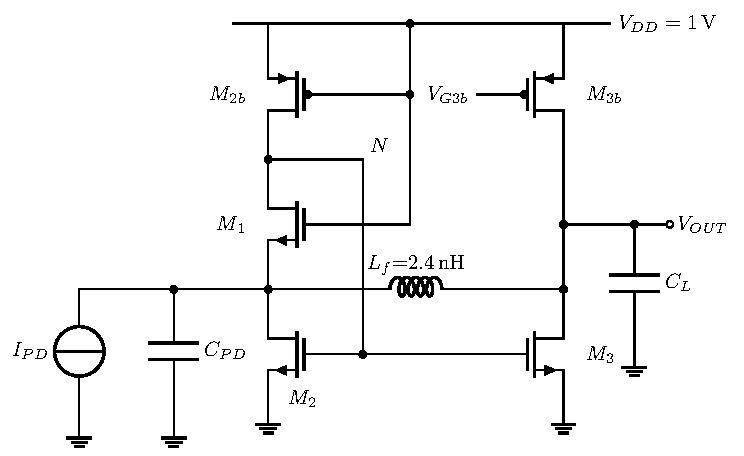
\includegraphics[width=0.47\linewidth]{figures/schem_baseline}\hfill
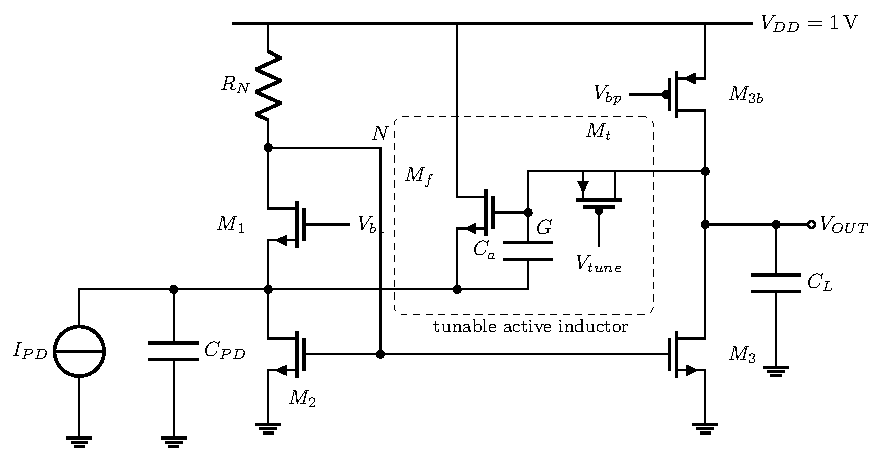
\includegraphics[width=0.52\linewidth]{figures/schem_proposed}
\caption{(a) Baseline TIA of \cite{baseline} with passive feedback inductor (left). (b) Proposed TIA with tunable active-inductor feedback (right). $V_{b1}$ and $V_{bp}$ come from the bias generator described in Section~\ref{sec:proposed}.}
\label{fig:schem}
\end{figure}

\subsection{Operating point and low-frequency gain}
With its gate at $V_{DD}$, $M_{2b}$ has zero gate-source voltage and conducts only leakage (\BIOne\,nA). $M_1$ therefore carries no bias current and sits in deep triode with a channel conductance of \BGdsOne\,mS: it is a switch that ties node $N$ to the input. The inductor is a DC short, so $M_2$ is diode-connected through $M_1$ and $L_f$, the input, $N$ and the output all rest at \BVin\,V, and the $M_{3b}$ current (\SI{1.32}{mA}) splits equally between $M_2$ and $M_3$.

For a feedback impedance $Z_f$ between output and input, and $v_N \approx v_{in}$, nodal analysis gives
\begin{equation}
Z_T(s)=\frac{v_{out}}{i_{in}}=\frac{1-g_{m3}Z_f}{(g_{m2}+g_{ds2})(1+g_oZ_f)+g_o+g_{m3}},\qquad g_o=g_{ds3}+g_{ds3b},
\label{eq:zt_base}
\end{equation}
when capacitances are neglected. At low frequency $Z_f\to 0$ and
\begin{equation}
Z_T(0)=\frac{1}{g_{m2}+g_{m3}+g_{ds2}+g_{ds3}+g_{ds3b}} .
\label{eq:zt0_base}
\end{equation}
With the simulated $g_{m2}=g_{m3}=\BGmTwo$\,mS, Eq.~\eqref{eq:zt0_base} evaluates to \BZtOhm\,$\Omega$ (\BZt\,dB$\Omega$), which is the simulated value. As $|Z_f|$ grows with frequency the feedback is removed and the gain rises towards $g_{m3}/(g_{m2}g_o)$; the inductor then resonates with the node capacitances.

\subsection{Simulated response and differences from the published curves}
Fig.~\ref{fig:baseline} compares the re-simulation with points digitised from Figs.~3 and~6 of \cite{baseline}. The re-simulated gain is \BZt\,dB$\Omega$ at low frequency, stays within $\pm\SI{1}{dB}$ up to \BFlat\,GHz and then rises to a peak \BPk\,dB above the low-frequency value at \BFpk\,GHz. The input-referred noise is \BInOne, \BInFive\ and \BInTen\,pA/$\sqrt{\text{Hz}}$ at 1, 5 and \SI{10}{GHz}, and the supply current is \SI{1.32}{mA}. With the $M_{3b}$ gate at \SI{-1}{V} the gain drops to \BMZt\,dB$\Omega$ and the power rises to \BMPow\,mW.

\begin{figure}[t]
\centering
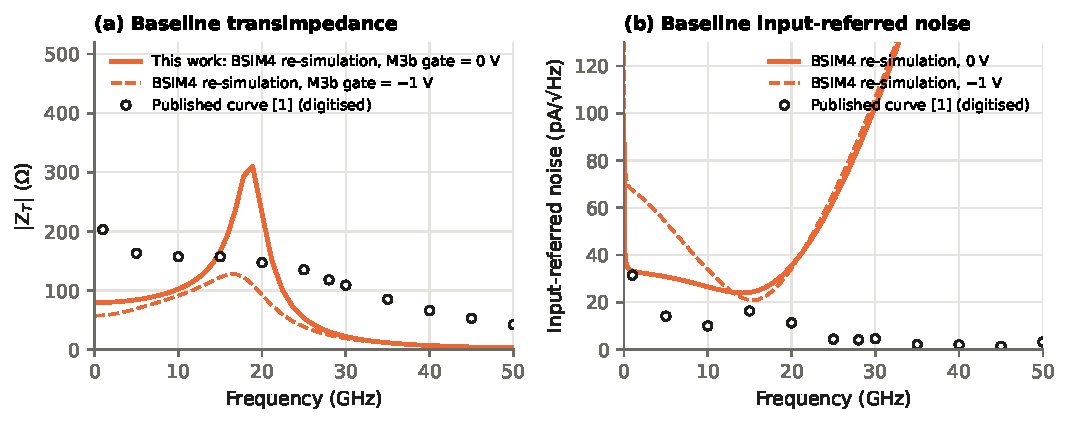
\includegraphics[width=0.95\linewidth]{figures/fig_baseline_reproduction}
\caption{Baseline TIA re-simulated with the 90\,nm PTM BSIM4 model, compared with points digitised from \cite{baseline}. The digitised points are approximate.}
\label{fig:baseline}
\end{figure}

The published curve is higher (about \SI{157}{\ohm} in band), shows no resonance and reports lower noise. The simulator, device model, capacitances and bias used in \cite{baseline} are not available, so the cause cannot be established; the published transfer function has a zero at the origin, which also differs from its plotted response. What can be said is narrower: with a model that enforces the threshold voltage, the schematic as drawn does not bias $M_1$ as a common-gate amplifier, and its response is a resonant peak, not a flat band. The re-simulated circuit is used as the reference for the rest of this paper.

\section{Proposed circuit}\label{sec:proposed}
\subsection{Topology and bias}
Fig.~\ref{fig:schem}(b) shows the proposed TIA. Three changes are made.

\emph{Input stage.} $M_{2b}$ is replaced by a resistor $R_N$, and the gate of $M_1$ is biased at $V_{b1}$ so that $M_1$ carries \IOne\,\si{\micro A} and operates in saturation. $M_1$ and $M_2$ then form a flipped voltage follower \cite{fvf}: $M_1$ senses the input node and drives the gate of $M_2$, which lowers the input resistance in the same way as a regulated cascode \cite{park}. The input rests at \Vin\,V, well below the \BVin\,V of the baseline, and this level shift is what makes room for the feedback device.

\emph{Loads.} $M_{3b}$ is a mirror of a reference current, so the output-branch current is set by $I_{ref}$ and not by the supply and threshold voltages. $V_{b1}$ is produced by a diode-connected replica of $M_1$ in series with a resistor $R_b$.

\emph{Feedback.} The spiral is replaced by the source follower $M_f$. Its source drives the input node, its drain is at $V_{DD}$, and its gate (node $G$) is connected to the output through the PMOS triode device $M_t$, whose gate is $V_{tune}$. A capacitor $C_a$ between gate and source adds to $C_{gs}$ of $M_f$. $M_f$ needs a gate-source drop of about \SI{0.4}{V}; with the input at \Vin\,V the output settles at \Vout\,V, which leaves \SI{0.34}{V} across $M_{3b}$. No DC current flows in $M_t$, so the tuning voltage does not disturb the operating point.

Table~\ref{tab:sizes} lists the device sizes. They were chosen with a differential-evolution search over widths, $R_N$, $R_b$ and $C_a$ that maximised bandwidth subject to at least \SI{53}{dB\ohm}, at most \SI{1}{dB} peaking, at most \SI{1.2}{mW} and every device in saturation, and were then rounded. The supply current is \ITot\,\si{\micro A}, of which \SI{97}{\micro A} is in the bias generator.

\begin{table}[t]
\centering
\caption{Device sizes of the proposed TIA ($W/L$ in \si{\micro m}). $R_N=\SI{5}{k\ohm}$, $R_b=\SI{4.2}{k\ohm}$, $C_a=\SI{30}{fF}$, $I_{ref}=\SI{50}{\micro A}$, decoupling on $V_{b1}$ \SI{2}{pF}.}
\label{tab:sizes}
\begin{tabular}{llll}
\toprule
Device & $W/L$ & Device & $W/L$ \\
\midrule
\tableinput table_sizes.tex 
\bottomrule
\end{tabular}
\end{table}

\subsection{Active-inductor impedance}
Seen from the input node with the output held at AC ground, $M_f$ and its gate network present
\begin{equation}
Z_{AI}(s)=\frac{1+sR_tC_g}{g_f+sC_g},\qquad g_f=g_{mf}+g_{mbf}+g_{dsf},\quad C_g=C_a+C_{gsf},
\label{eq:zai}
\end{equation}
where $R_t$ is the channel resistance of $M_t$. This is the classical single-transistor active inductor \cite{yuan,sackingerla}: a series resistance $R_s=1/g_f$ and, below the pole at $g_f/C_g$, an equivalent inductance
\begin{equation}
L_{eq}=\frac{C_g}{g_f}\left(R_t-\frac{1}{g_f}\right).
\label{eq:leq}
\end{equation}
The element is inductive only when $R_t>1/g_f$; below that it is a resistance shunted by a capacitance. Unlike the spiral it is unilateral: the current it delivers to the input is controlled by the output voltage, but it draws no signal current from the output node. It is therefore an active feedback path with an inductive transfer admittance, not a two-terminal floating inductor.

\subsection{Small-signal transimpedance}
Let $m=g_{m3}/g_{m2}$ be the mirror current gain, $R_o=1/(g_{ds3}+g_{ds3b})$ the output resistance and $A_1=(g_{m1}+g_{mb1}+g_{ds1})/(1/R_N+g_{ds1})$ the gain from the input to node $N$. At low frequency, when $A_1\gg 1$,
\begin{equation}
Z_T(0)\approx-\frac{mR_o}{1+T_0},\qquad T_0=m\,g_{mf}R_o ,
\label{eq:zt0}
\end{equation}
and, with the output capacitance $C_o$ and the feedback admittance $g_{mf}/(1+sR_tC_g)$,
\begin{equation}
Z_T(s)\approx-\frac{mR_o\,(1+sR_tC_g)}{(1+sR_oC_o)(1+sR_tC_g)+T_0}\,H_{in}(s),
\label{eq:zt}
\end{equation}
where $H_{in}(s)$ is the second-order response of the flipped-voltage-follower stage, with natural frequency close to $\sqrt{g_{m1}g_{m2}/(C_{in}C_N)}$. The gate network places a zero at $1/(R_tC_g)$ in the closed-loop response and turns the output pole into a pair whose damping falls as $R_t$ rises. $V_{tune}$ therefore sets how fast the feedback is removed with frequency: a small $R_t$ gives a response that droops early, a larger one flattens it, and a still larger one peaks.

With the simulated operating point ($m=\Mratio$, $R_o=\Ro\,\Omega$, $g_{mf}=\GmF$\,mS, $A_1=\AOne$), Eq.~\eqref{eq:zt0} gives $T_0=\Tzero$ and $|Z_T(0)|=\ZtApprox\,\Omega$; the expression without the $A_1\gg1$ approximation gives \ZtExact\,$\Omega$, and SPICE gives \PZtOhm\,$\Omega$.

\subsection{Noise}
To first order the input-referred noise current density is
\begin{equation}
\overline{i_{n}^2}\approx 4kT\left[\gamma\left(g_{m2}+g_{mf}\right)+\frac{1}{R_N}+\frac{\gamma\left(g_{m3}+g_{m3b}\right)}{m^2}\right]+4kT\gamma g_{m1}\left(\frac{\omega C_{in}}{g_{m1}}\right)^2 ,
\label{eq:noise}
\end{equation}
where $C_{in}$ is the total input capacitance. $M_2$, $M_f$ and $R_N$ inject directly at the input, the output-branch devices are divided by the mirror gain, and the common-gate device contributes in proportion to $\omega^2$. Eq.~\eqref{eq:noise} is given to identify the terms; the simulated budget in Section~\ref{sec:results} is the quantitative statement.

\section{Simulation results}\label{sec:results}
\subsection{Gain, bandwidth and noise at the nominal setting}
Fig.~\ref{fig:compare} compares the two circuits at $V_{tune}=\VtNom$\,V. The proposed TIA has \PZt\,dB$\Omega$ (\PZtOhm\,$\Omega$) at low frequency, a $-3$\,dB bandwidth of \PBW\,GHz and \PPk\,dB peaking, and it draws \PPow\,mW. The input-referred noise is \PInOne, \PInFive\ and \PInTen\,pA/$\sqrt{\text{Hz}}$ at 1, 5 and \SI{10}{GHz}; integrated over the bandwidth it is \PIrms\,\si{\micro A} rms, and the total output noise divided by the low-frequency gain is \PIrmsTot\,\si{\micro A} rms. For a bit-error ratio of $10^{-12}$ ($Q=7.03$) this corresponds to a minimum input swing of \SensIpp\,\si{\micro A} peak to peak, or \SensdBm\,dBm average optical power for an assumed responsivity of \SI{0.8}{A/W} and an ideal extinction ratio.

\begin{figure}[t]
\centering
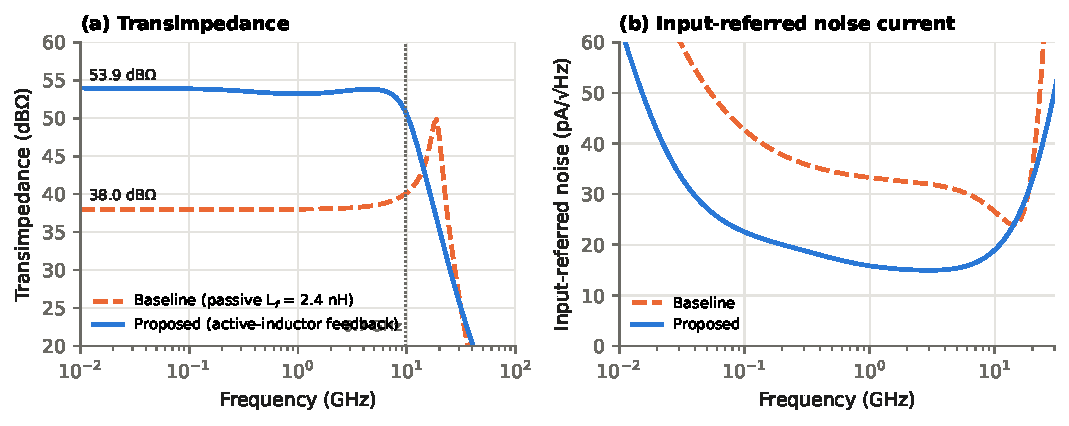
\includegraphics[width=0.95\linewidth]{figures/fig_baseline_vs_proposed}
\caption{Re-simulated baseline and proposed TIA under identical conditions ($C_{PD}=\SI{50}{fF}$, $C_L=\SI{30}{fF}$, \SI{1}{V}, \SI{35}{\celsius}).}
\label{fig:compare}
\end{figure}

Fig.~\ref{fig:noise} gives the noise by device. At \SI{5}{GHz} the common-gate device $M_1$ contributes \NsMOne\,\% of the output noise power, $M_2$ \NsMTwo\,\%, $M_3$ \NsMThree\,\%, the feedback follower $M_f$ \NsMf\,\%, the tuning device $M_t$ \NsMt\,\%, $R_N$ \NsRn\,\% and $M_{3b}$ \NsMThreeB\,\%. The feedback network, the part that replaces the spiral, therefore accounts for about one fifth of the noise power. In the baseline the triode device $M_1$ alone contributes \NsBMOne\,\%, which is why the baseline is noisier although it has fewer devices.

\begin{figure}[t]
\centering
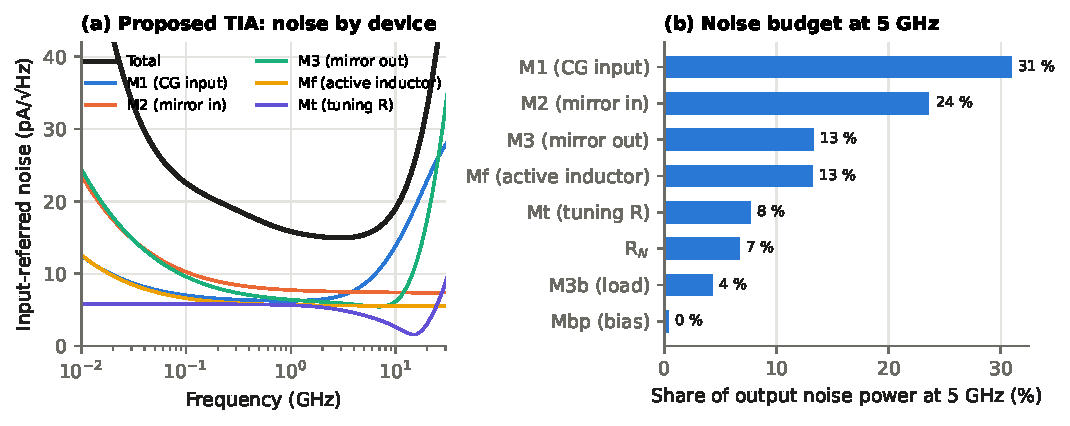
\includegraphics[width=0.95\linewidth]{figures/fig_noise}
\caption{Proposed TIA: (a) input-referred noise by device, (b) share of output noise power at \SI{5}{GHz}.}
\label{fig:noise}
\end{figure}

\subsection{Active inductor on its own}
Fig.~\ref{fig:ai} shows $Z_{AI}$ simulated at the bias point of the TIA for several tuning voltages. The low-frequency resistance is \AIRs\,$\Omega$ ($g_{mf}=\AIgm$\,mS). Eq.~\eqref{eq:leq} places the boundary between capacitive and inductive behaviour at $R_t=1/g_f$, which is reached near \SI{0.24}{V}; in simulation the impedance turns inductive slightly later, at about \SI{0.27}{V}. At \SI{1}{GHz} the simulated equivalent inductance is \AILA, \AILB, \AILC\ and \AILD\,nH at $V_{tune}=0.28$, 0.32, 0.36 and \SI{0.40}{V}, with a peak quality factor of \AIQD\ at \SI{0.40}{V}. This is a very lossy inductor; its use here is as a tunable zero, not as a resonator. Eq.~\eqref{eq:leq} overestimates $L_{eq}$ by a factor of two to three, which is attributed to capacitance at node $G$ that the first-order expression ignores.

\begin{figure}[t]
\centering
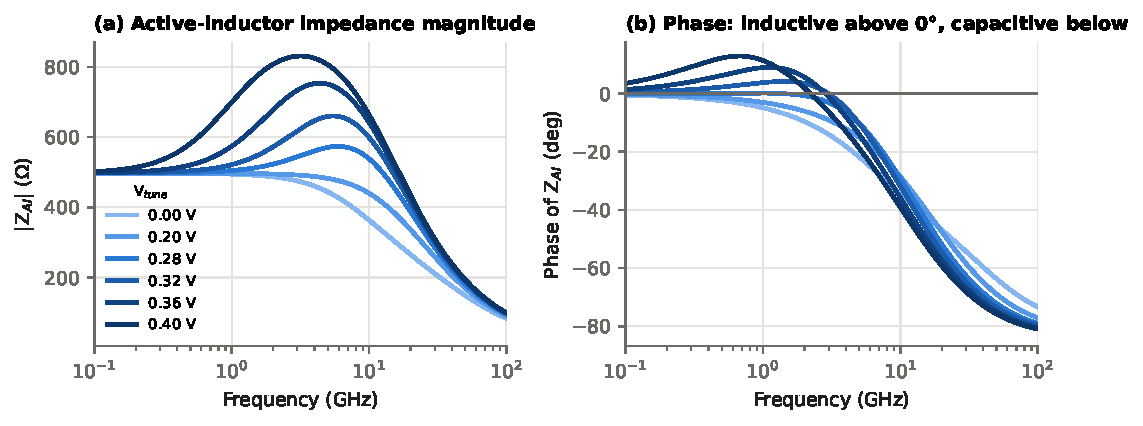
\includegraphics[width=0.95\linewidth]{figures/fig_active_inductor}
\caption{Simulated impedance of the active inductor seen from the input node with the output at AC ground.}
\label{fig:ai}
\end{figure}

\subsection{Tuning law}
Fig.~\ref{fig:tune} and Table~\ref{tab:tune} give the response as $V_{tune}$ is swept. $R_t$ changes from \RtMin\,$\Omega$ at \SI{0}{V} to \RtMaxOne\,$\Omega$ at \VtOneDb\,V. Over that range the bandwidth moves from \TuneMin\ to \TuneMax\,GHz, a ratio of \TuneRatio, while the peaking stays below \SI{1}{dB} and the low-frequency gain does not change. Above \VtOneDb\,V the bandwidth saturates and the peaking grows, reaching \PkMax\,dB at \VtMax\,V. The integrated input noise falls from \PIrms\ to \IrmsMin\,\si{\micro A} at the lowest setting, so a lower data rate can be received with a smaller noise bandwidth.

\begin{figure}[t]
\centering
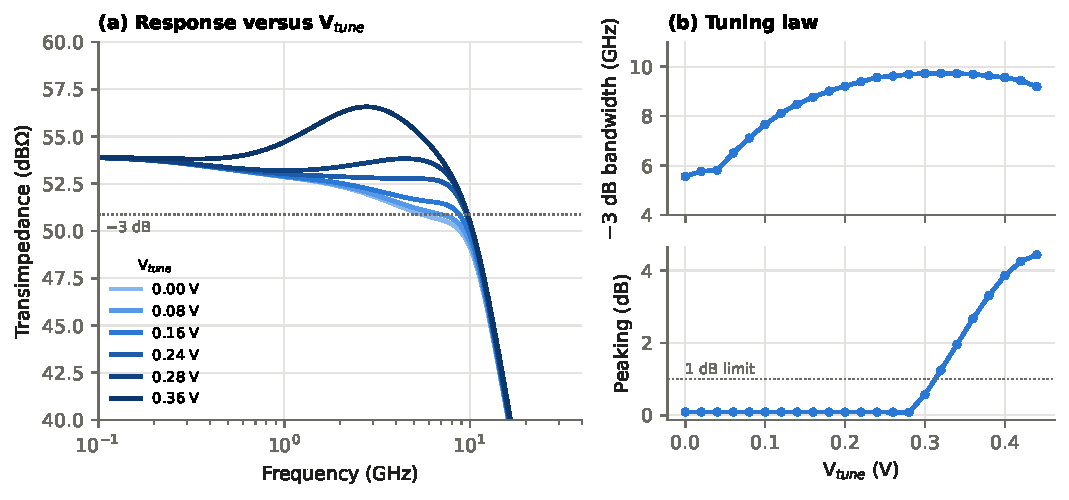
\includegraphics[width=0.95\linewidth]{figures/fig_vtune_tuning}
\caption{Proposed TIA versus tuning voltage: (a) transimpedance, (b) $-3$\,dB bandwidth and peaking.}
\label{fig:tune}
\end{figure}

\begin{table}[t]
\centering
\caption{Tuning law of the proposed TIA (nominal process, \SI{1}{V}, \SI{35}{\celsius}).}
\label{tab:tune}
\begin{tabular}{cccccc}
\toprule
$V_{tune}$ (V) & $R_t$ ($\Omega$) & BW (GHz) & Peaking (dB) & $i_{n,rms}$ (\si{\micro A}) & $i_n$ at \SI{5}{GHz} (pA/$\sqrt{\text{Hz}}$) \\
\midrule
\tableinput table_tune.tex 
\bottomrule
\end{tabular}
\end{table}

\subsection{Reduced-order model}
The four-node small-signal model behind Eq.~\eqref{eq:zt} (nodes: input, $N$, output, $G$) was evaluated with the conductances of the simulated operating point and six effective capacitances fitted to the SPICE response at $V_{tune}=0$ and \SI{0.28}{V} only. Fig.~\ref{fig:model} compares it with SPICE. Up to \SI{30}{GHz} the rms error is at most \ModelRmsLow\,dB (\ModelMaxLow\,dB maximum) for the settings up to \SI{0.28}{V}, including the two that were not used in the fit, and \ModelRmsMax\,dB rms (\ModelMaxAll\,dB maximum) at \SI{0.36}{V}. The fitted capacitances are effective values that absorb distributed effects, and the model predicts the $-3$\,dB frequency less well than the curve where the roll-off is shallow; it is offered as a design aid, not as a substitute for simulation.

\begin{figure}[t]
\centering
\begin{minipage}{0.48\linewidth}\centering
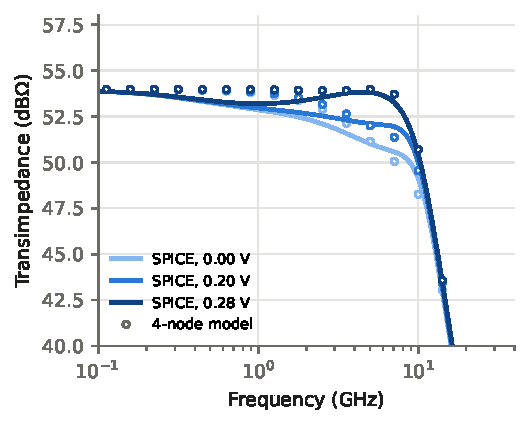
\includegraphics[width=\linewidth]{figures/fig_model_vs_spice}
\caption{Four-node model (markers) against SPICE (lines).}
\label{fig:model}
\end{minipage}\hfill
\begin{minipage}{0.48\linewidth}\centering
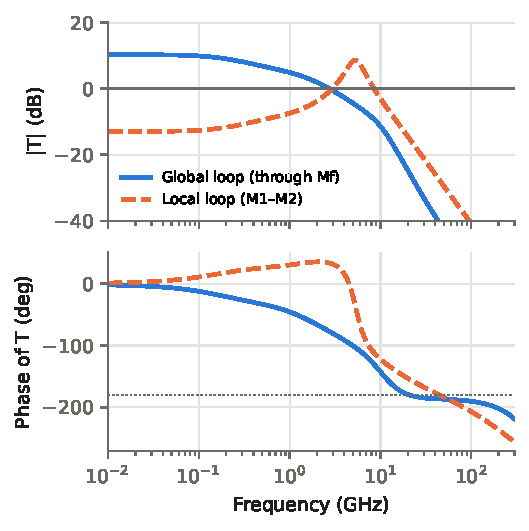
\includegraphics[width=\linewidth]{figures/fig_loop_gain}
\caption{Loop gains at the nominal setting.}
\label{fig:loop}
\end{minipage}
\end{figure}

\subsection{Stability}
Loop gains were obtained with Middlebrook's double-injection method \cite{middlebrook}, which remains valid when the break point is loaded on both sides. The global loop, broken between the output and $M_t$, has a low-frequency gain of \LoopTzero\,dB and crosses unity between \LoopFuMin\ and \LoopFuMax\,GHz with at least \LoopPMg\si{\degree} of phase margin over the tuning range. The local loop of the flipped voltage follower, broken at the gate of $M_2$ with the global loop closed, has a phase margin of at least \LoopPMl\si{\degree} over the tuning range at $C_{PD}=\SI{50}{fF}$ and \LoopPMlCpd\si{\degree} at \SI{200}{fF} (Fig.~\ref{fig:loop}). The local loop is the one that limits stability, and its margin falls as the photodiode capacitance rises.

\subsection{Process, voltage and temperature}
The PTM card has no foundry corners. Corners were emulated by shifting the threshold voltage by $\pm\SI{30}{mV}$ and the mobility by $\pm\SI{5}{\percent}$, separately for NMOS and PMOS; resistors were varied by $\pm\SI{15}{\percent}$ and $C_a$ by $\pm\SI{10}{\percent}$. Table~\ref{tab:pvt} and Fig.~\ref{fig:pvt} report fifteen conditions, first with $V_{tune}$ fixed at \VtNom\,V and then with $V_{tune}$ chosen, on a \SI{20}{mV} grid, as the setting with at most \SI{0.5}{dB} peaking whose bandwidth is closest to the nominal \PBW\,GHz.

With a fixed setting the bandwidth spans \PvtBwMin\ to \PvtBwMax\,GHz and the peaking reaches \PvtPkMax\,dB. After trimming the peaking is at most \PvtPkTMax\,dB and the bandwidth spans \PvtBwTMin\ to \PvtBwTMax\,GHz. Trimming removes peaking and pulls fast conditions back to the target, but it cannot restore bandwidth that the input stage has lost: at \SI{85}{\celsius}, and in the slow, low-voltage, hot condition, the bandwidth stays below nominal. The gain stays between \PvtZtMin\ and \PvtZtMax\,dB$\Omega$ and the power between \PvtPMin\ and \PvtPMax\,mW.

\begin{table}[t]
\centering
\caption{Process, voltage and temperature results. Corners are emulated parameter skews, not foundry corners.}
\label{tab:pvt}
\begin{tabular}{lccccc}
\toprule
 & \multicolumn{2}{c}{$V_{tune}=\VtNom$\,V} & \multicolumn{3}{c}{$V_{tune}$ trimmed} \\
\cmidrule(lr){2-3}\cmidrule(lr){4-6}
Condition & BW (GHz) & Peaking (dB) & $V_{tune}$ (V) & BW (GHz) & Peaking (dB) \\
\midrule
\tableinput table_pvt.tex 
\bottomrule
\end{tabular}
\end{table}

\begin{figure}[t]
\centering
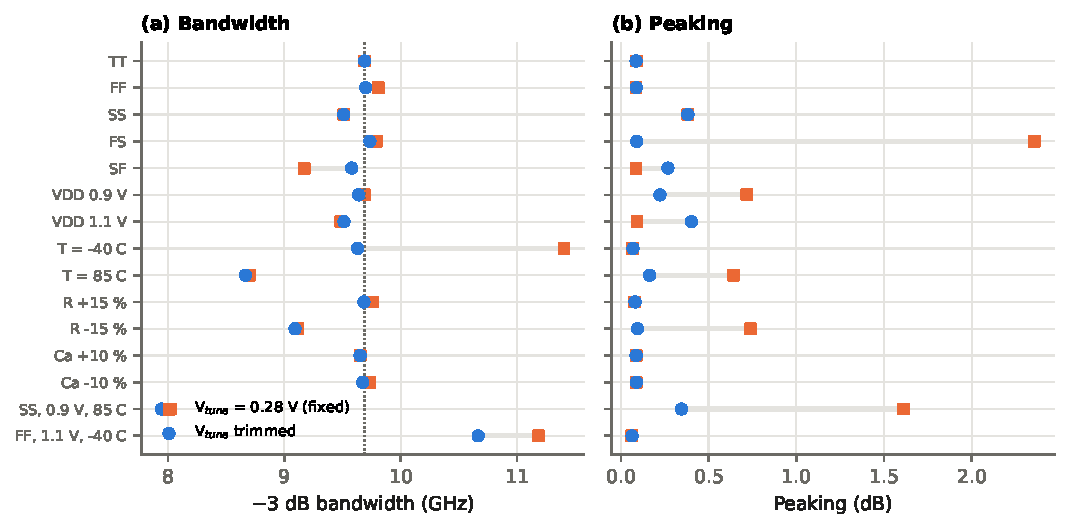
\includegraphics[width=0.95\linewidth]{figures/fig_pvt}
\caption{Bandwidth and peaking over fifteen conditions with a fixed and a trimmed tuning voltage. The dotted line marks the nominal bandwidth.}
\label{fig:pvt}
\end{figure}

\subsection{Monte Carlo}
A \McN-sample Monte Carlo run combined global variation (threshold $\sigma=\SI{10}{mV}$, mobility $\sigma=\SI{2}{\percent}$, resistors $\sigma=\SI{5}{\percent}$, $C_a$ $\sigma=\SI{3}{\percent}$) with local mismatch following Pelgrom's law \cite{pelgrom} ($A_{VT}=\SI{3.5}{mV.\micro m}$, $A_\beta=\SI{1}{\percent.\micro m}$). These coefficients are assumed typical values for the node, not extracted data. With $V_{tune}$ fixed the bandwidth is $\McBwMean\pm\McBwStd$\,GHz (mean $\pm$ one standard deviation; range \McBwMin\ to \McBwMax\,GHz) and the worst peaking is \McPkMax\,dB; \McPkYieldFixed\,\% of samples have at most \SI{1}{dB} peaking. With the same trimming rule as above the bandwidth is $\McBwTMean\pm\McBwTStd$\,GHz, the worst peaking is \McPkTMax\,dB and every sample meets the \SI{1}{dB} limit; the trim voltages lie between \McVtMin\ and \McVtMax\,V. The low-frequency gain is $\McZtMean\pm\McZtStd$\,dB$\Omega$ (Fig.~\ref{fig:mc}).

\begin{figure}[t]
\centering
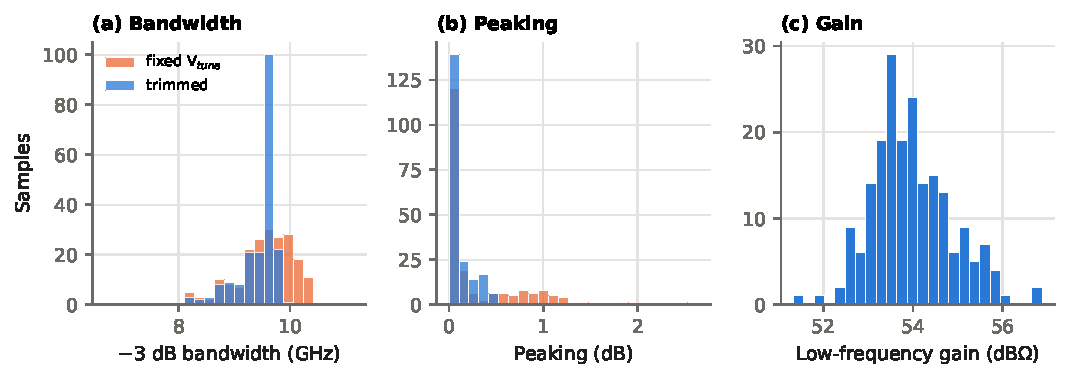
\includegraphics[width=0.95\linewidth]{figures/fig_monte_carlo}
\caption{Monte Carlo distributions (\McN\ samples) with a fixed and a trimmed tuning voltage.}
\label{fig:mc}
\end{figure}

\subsection{Transient response}
Fig.~\ref{fig:eye} shows eye diagrams for a $2^7-1$ pseudo-random sequence with a \SI{100}{\micro A} peak-to-peak input, the test current used in \cite{baseline}, and a rise time of a quarter of the bit period. No noise is included. At \SI{10}{Gb/s} the proposed TIA produces a \EyePTenAmp\,mV output swing with a vertical opening of \EyePTenH\,mV (\EyePTenPct\,\% of the swing) and a horizontal opening of \EyePTenW\,\% of the unit interval; the baseline produces \EyeBTenH\,mV. At \SI{12.5}{Gb/s} the proposed TIA keeps \EyePTwH\,mV and \EyePTwW\,\%, while the baseline's horizontal opening falls to \EyeBTwW\,\% because of ringing at its resonance.

\begin{figure}[t]
\centering
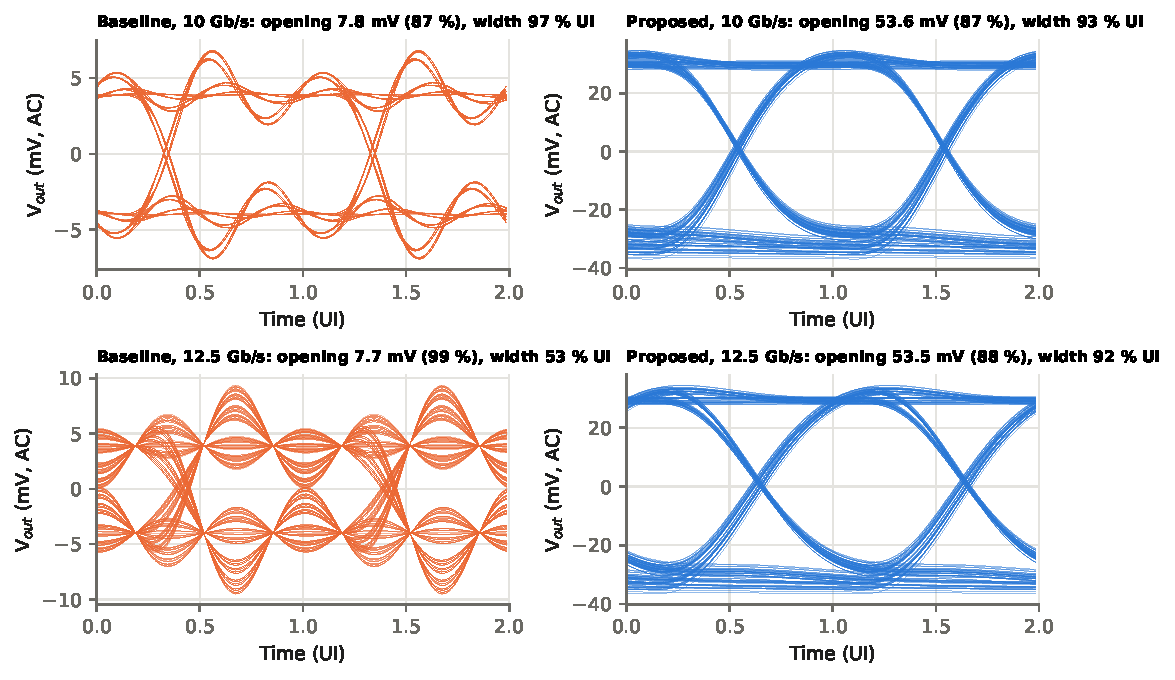
\includegraphics[width=0.95\linewidth]{figures/fig_eye_diagrams}
\caption{Simulated eye diagrams, \SI{100}{\micro A} peak-to-peak input, no noise.}
\label{fig:eye}
\end{figure}

\subsection{Load, photodiode capacitance and input overload}
Fig.~\ref{fig:load}(a) and Table~\ref{tab:load} compare the active-inductor network with plain follower feedback, in which the gate of $M_f$ is tied directly to the output and $C_a$ is removed. At the nominal \SI{30}{fF} load the plain follower is faster, \LdResLight\ against \LdAiLight\,GHz, because the bandwidth is then set by the input stage and the tuning network only adds capacitance. As the load grows the output pole becomes dominant and the inductive zero recovers part of the loss: the ratio is \LdRatioMid\ at \SI{150}{fF} and \LdRatioHeavy\ at \SI{250}{fF} (\LdAiHeavy\ against \LdResHeavy\,GHz).

Fig.~\ref{fig:load}(b) shows the effect of the photodiode capacitance. With a fixed setting the peaking grows with $C_{PD}$; lowering $V_{tune}$ brings it back below \SI{1}{dB} up to \SI{200}{fF}, at a bandwidth of about \SI{7.4}{GHz}.

Fig.~\ref{fig:load}(c) shows the small-signal gain against a DC input current. The follower $M_f$ carries \IF\,\si{\micro A}, and photocurrent sourced into the input displaces it. The gain rises by \OvA\,dB at \SI{25}{\micro A} and \OvB\,dB at \SI{50}{\micro A}, where the bandwidth has fallen to \OvBwB\,GHz, and the feedback is lost near \SI{100}{\micro A}, where $M_f$ is starved. The baseline gain changes by less than \SI{1.3}{dB} up to \SI{1}{mA}.

\begin{figure}[t]
\centering
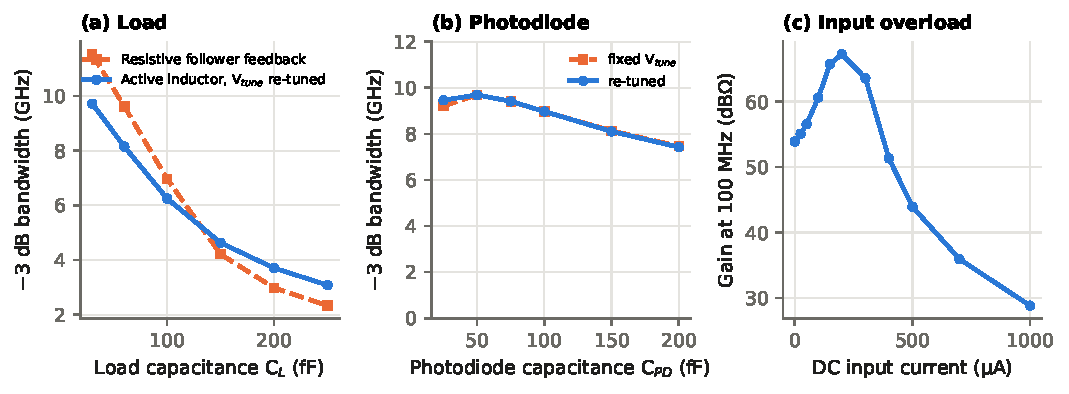
\includegraphics[width=0.98\linewidth]{figures/fig_load_pd_overload}
\caption{(a) Bandwidth against load for plain follower feedback and for the active inductor with $V_{tune}$ re-tuned for at most \SI{1}{dB} peaking. (b) Bandwidth against photodiode capacitance. (c) Gain at \SI{100}{MHz} against DC input current.}
\label{fig:load}
\end{figure}

\begin{table}[t]
\centering
\caption{Bandwidth (GHz) of plain follower feedback and of the active-inductor network against load capacitance.}
\label{tab:load}
\begin{tabular}{cccccc}
\toprule
$C_L$ (fF) & Plain follower & AI, $V_{tune}=\VtNom$\,V & Best $V_{tune}$ (V) & AI, re-tuned & Ratio \\
\midrule
\tableinput table_load.tex 
\bottomrule
\end{tabular}
\end{table}

\section{Discussion}\label{sec:discussion}
\subsection{What the active inductor does and does not do}
The simulations support four statements. (i) The feedback element needs no spiral. A \SI{2.4}{nH} square spiral with 3.5 turns, \SI{6}{\micro m} tracks and \SI{2}{\micro m} spacing has an outer side of about \SpiralSide\,\si{\micro m} by the modified Wheeler expression \cite{mohanl}, or \SpiralArea\,mm$^2$. $M_f$, $M_t$ and a \SI{30}{fF} capacitor at an assumed \SI{1.5}{fF/\micro m^2} occupy about \AIArea\,\si{\micro m^2} when a five-fold allowance is made for contacts, spacing and routing, a ratio of roughly \AreaRatio. Both figures are estimates from dimensions, not layouts. (ii) One control voltage moves the bandwidth over a \TuneRatio:1 range at constant gain. (iii) The same voltage removes peaking caused by process, supply, temperature and photodiode spread. (iv) For loads of \SI{150}{fF} and above the inductive zero extends the bandwidth beyond that of resistive feedback.

They also support three limits. The network does not raise the maximum bandwidth at light loads; a designer who needs neither tuning nor trimming is better served by tying the follower gate to the output. Trimming cannot recover bandwidth lost by the input stage in slow or hot conditions. And the price of tunability at the nominal load is about \SI{16}{\percent} of bandwidth relative to the plain follower.

\subsection{Comparison}
Table~\ref{tab:comp} places the result beside the baseline and related current-mirror and tunable TIAs. The figures for other works are those their authors report, under their own conditions, and are not re-simulated here. Against the re-simulated baseline under identical conditions the proposed circuit has \GainImp\,dB more gain, \NoiseRatio\ times lower noise density at \SI{5}{GHz}, \PowSave\,\% lower power and a flat response in place of a resonance.

\begin{table}[t]
\centering
\caption{Comparison with the baseline and related work. n/r: not reported.}
\label{tab:comp}
\footnotesize\setlength{\tabcolsep}{3.5pt}
\begin{tabular}{lllllll}
\toprule
Work & Process, supply & Gain (dB$\Omega$) & BW (GHz) & Power (mW) & Inductor & Tunable \\
\midrule
\cite{baseline}, as published & 90\,nm, \SI{1}{V} & 43.92 & 5--15 (flat) & n/r & spiral, \SI{2.4}{nH} & no \\
\cite{baseline}, re-simulated & 90\,nm PTM, \SI{1}{V} & \BZt & \BFlat\ ($\pm$\SI{1}{dB}) & \BPow & spiral, \SI{2.4}{nH} & no \\
\cite{zohoori} & 90\,nm, \SI{1}{V} & 40.5 & 7 & 1.4 & none & no \\
\cite{hassan} & n/r & 57.5 & 6.6 & n/r & none & no \\
\cite{issa} & 45\,nm, \SI{1}{V} & 68.2 & 2.5 & n/r & active, local & no \\
\cite{alyas} & 45\,nm, \SI{1}{V} & 62.2 & 1 & n/r & active, local & not swept \\
\cite{hwang} & \SI{0.18}{\micro m} & 52 & 3.9--7.6 & n/r & none & yes \\
This work (simulated) & 90\,nm PTM, \SI{1}{V} & \PZt & \TuneMin--\TuneMax & \PPow & active, global & yes \\
\bottomrule
\end{tabular}
\end{table}

\subsection{Limitations}
The results are schematic-level simulations with a predictive model. Layout parasitics, especially at the input and at node $N$, will lower the bandwidth, and the synthetic corners and assumed mismatch coefficients stand in for foundry data. The photodiode is a current source with a capacitor; bond-wire or bump inductance and electrostatic-discharge protection are not modelled. The reference current is ideal. The input stage tolerates only a few tens of microamperes of average photocurrent, so a practical receiver needs a DC-cancellation loop at the input or a larger follower current, at a cost in noise or gain. The \SI{37}{mV} saturation margin of $M_{3b}$ is small. The eye diagrams contain no noise. Each of these is a necessary next step before the circuit could be claimed to be ready for fabrication.

\section{Conclusion}
A published 90\,nm current-mirror TIA with a spiral feedback inductor was re-simulated with a BSIM4 model and found to give \BZt\,dB$\Omega$ with an \BPk\,dB resonance, because its common-gate device is left in triode. A replacement was designed in which the input devices form a flipped voltage follower and the feedback path is a source follower with a voltage-tuned gate network. In simulation at \SI{1}{V} and \PPow\,mW it reaches \PZt\,dB$\Omega$, \PBW\,GHz and \PInFive\,pA/$\sqrt{\text{Hz}}$ at \SI{5}{GHz} without an inductor, its bandwidth can be set between \TuneMin\ and \TuneMax\,GHz by one voltage, and the same voltage holds peaking at or below \SI{0.5}{dB} across the process, voltage, temperature and mismatch cases examined. The tuning network does not extend the maximum bandwidth at light loads and the input overloads at a few tens of microamperes of average current; a DC-cancellation loop, post-layout verification with a foundry kit and measurement are the next steps.

\section*{Data availability}
The netlists, the model card, the scripts that run every simulation and the raw results are available in the project repository.

\begin{thebibliography}{99}
\bibitem{razavi} B. Razavi, \emph{Design of Integrated Circuits for Optical Communications}, 2nd ed. Hoboken, NJ, USA: Wiley, 2012.
\bibitem{sackinger} E. S\"ackinger, \emph{Analysis and Design of Transimpedance Amplifiers for Optical Receivers}. Hoboken, NJ, USA: Wiley, 2017.
\bibitem{zohoori} S. Zohoori, M. Dolatshahi, M. Pourahmadi, and M. Hajisafari, ``A CMOS low-power current-mirror-based transimpedance amplifier for 10 Gbps optical communications,'' \emph{Microelectron. J.}, vol. 80, pp. 18--27, 2018.
\bibitem{hassan} M. Hassan and H. Zimmermann, ``A 10Gb/s inductor less push pull current mirror transimpedance amplifier,'' in \emph{Proc. 19th IEEE Int. Conf. Electronics, Circuits, and Systems (ICECS)}, Seville, Spain, 2012.
\bibitem{atef} M. Atef, ``High gain transimpedance amplifier with current mirror load,'' in \emph{Proc. 21st Int. Conf. Mixed Design of Integrated Circuits and Systems (MIXDES)}, Lublin, Poland, 2014.
\bibitem{issa} M. S. H. Alsheikhjader and A. A. Issa, ``A simulated 45 nm MOSFET channel process in transimpedance amplifier design for optoelectronics applications,'' \emph{Jordan J. Phys.}, vol. 17, no. 2, pp. 165--178, 2024.
\bibitem{alyas} M. M. Alyas and M. S. H. Alsheikhjader, ``A low-power 45 nm CMOS transimpedance amplifier with active inductor feedback for fiber-optic applications,'' \emph{Jordan J. Phys.}, vol. 19, no. 2, pp. 131--143, 2026.
\bibitem{abdalla} Y. S. M. Abdalla, ``Design of a novel CMOS transimpedance amplifier based on a current mirror,'' \emph{Int. J. Circuit Theory Appl.}, 2024, doi: 10.1002/cta.4353.
\bibitem{mohanbw} S. S. Mohan, M. del M. Hershenson, S. P. Boyd, and T. H. Lee, ``Bandwidth extension in CMOS with optimized on-chip inductors,'' \emph{IEEE J. Solid-State Circuits}, vol. 35, no. 3, pp. 346--355, 2000.
\bibitem{yuan} F. Yuan, \emph{CMOS Active Inductors and Transformers: Principle, Implementation, and Applications}. New York, NY, USA: Springer, 2008.
\bibitem{sackingerla} E. S\"ackinger and W. C. Fischer, ``A 3-GHz 32-dB CMOS limiting amplifier for SONET OC-48 receivers,'' \emph{IEEE J. Solid-State Circuits}, vol. 35, no. 12, pp. 1884--1888, 2000.
\bibitem{hwang} H.-Y. Hwang, J.-C. Chien, T.-Y. Chen, and L.-H. Lu, ``A CMOS tunable transimpedance amplifier,'' \emph{IEEE Microw. Wireless Compon. Lett.}, vol. 16, no. 12, pp. 693--695, 2006.
\bibitem{baseline} M. S. H. Alsheikhjader, ``Low noise with wide band transimpedance amplifier for nonlinear fiber optical applications,'' \emph{Rafidain J. Sci.}, vol. 29, no. 1, pp. 71--78, 2020, doi: 10.33899/rjs.2020.164476.
\bibitem{ngspice} H. Vogt \emph{et al.}, \emph{Ngspice User's Manual}, version 42, 2023.
\bibitem{ptm} W. Zhao and Y. Cao, ``New generation of predictive technology model for sub-45 nm early design exploration,'' \emph{IEEE Trans. Electron Devices}, vol. 53, no. 11, pp. 2816--2823, 2006.
\bibitem{fvf} R. G. Carvajal \emph{et al.}, ``The flipped voltage follower: a useful cell for low-voltage low-power circuit design,'' \emph{IEEE Trans. Circuits Syst. I}, vol. 52, no. 7, pp. 1276--1291, 2005.
\bibitem{park} S. M. Park and H.-J. Yoo, ``1.25-Gb/s regulated cascode CMOS transimpedance amplifier for Gigabit Ethernet applications,'' \emph{IEEE J. Solid-State Circuits}, vol. 39, no. 1, pp. 112--121, 2004.
\bibitem{middlebrook} R. D. Middlebrook, ``Measurement of loop gain in feedback systems,'' \emph{Int. J. Electron.}, vol. 38, no. 4, pp. 485--512, 1975.
\bibitem{pelgrom} M. J. M. Pelgrom, A. C. J. Duinmaijer, and A. P. G. Welbers, ``Matching properties of MOS transistors,'' \emph{IEEE J. Solid-State Circuits}, vol. 24, no. 5, pp. 1433--1439, 1989.
\bibitem{mohanl} S. S. Mohan, M. del M. Hershenson, S. P. Boyd, and T. H. Lee, ``Simple accurate expressions for planar spiral inductances,'' \emph{IEEE J. Solid-State Circuits}, vol. 34, no. 10, pp. 1419--1424, 1999.
\end{thebibliography}

\end{document}
